\section{Neurophenomenology of KT}


\begin{frame}[label=ladila]{The dimensions of structured experience}
  
 \begin{center}%\includegraphics[height=1.2cm]{COPL}%
  %\hspace{2cm}
  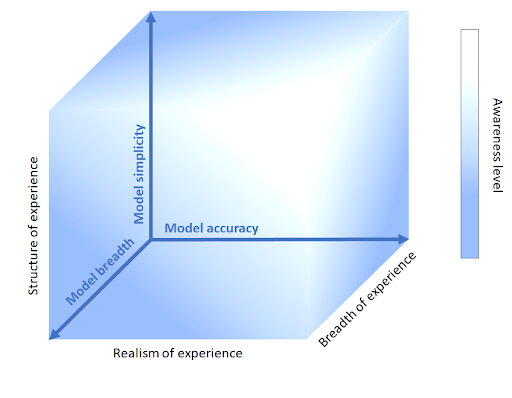
\includegraphics[height=7cm]{img/3dKT.png}
  \end{center}
  
   %Model features (simplicity, breadth, and accuracy) vs. neurophenomenology in KT. The panel displays objective model aspects, i.e., how simple/short the model/program is, how much data from input/output interfaces of the agent it tries to account for, and how well it matches data; and how these dimensions map into the level of \SEP (called awareness in the colorbar).
 
\end{frame}

%%%%%%%%%%%%%%%%%%%%%%%%%%%%%%%%%%%%%%%%%%%%%%%%%%%%%%%%%%%%%%%%%%%
\begin{frame}[label=ladila]{Altered states}
  
 Neurophenomenology defines a methodological strategy for integrating phenomenological and neurobiological accounts under one research program, by bridging  two irreducible phenomenal domains: 1P  (phenomenology, subjective measures) and 3P (physiology, objective measures) data \citep{Varela:1996aa}. \vfill
 
 Altered states of consciousness such as psychedelics or meditation offer an interesting context to study the effect of perturbing the mechanisms of \SEP.\vfill
 
Meditative states are associated with the global dissolution of the embodied self  \citep{Millire2018} and can  serve as unique models for a neurophenomenological investigation of self-dissolution (disengagement of self-models).\vfill
 
 As an  objective measure of structured experience, we can analyze descriptive narratives in speech form through state-of-the-art computational analysis (NLP) to establish  metrics on text structure such as semantic coherence and speech disorganization index~\citep{Sanz:2021, Tagliazucchi:2022, Mota:2017}.
 
 
\end{frame}


